\documentclass[]{csbsjuthesis}

\usepackage{algorithmic}
\usepackage{algorithm}
\usepackage{amsmath}
\usepackage{amssymb}
\usepackage{amsthm}
\usepackage{etoolbox}
\usepackage[hidelinks]{hyperref}
\usepackage{ifdraft}
\usepackage{listings}
\usepackage{mathtools}
\usepackage{pgfplots}
	\pgfplotsset{compat=1.16}
\usepackage{csvsimple}
\usepackage{siunitx}
\usepackage{subcaption}
\usepackage[obeyFinal]{todonotes}


%math typeseting
\newcommand{\mat}[1]{\mathbf{#1}}
\DeclarePairedDelimiter\ceil{\lceil}{\rceil}
\DeclarePairedDelimiter\floor{\lfloor}{\rfloor}
\renewcommand\qedsymbol{$\blacksquare$}

%setup todo notes
%note that notes are hidden in draft mode to improve compile times
\newcommand{\review}[1]{\ifdraft{}{\todo[linecolor=yellow,backgroundcolor=yellow!25,bordercolor=yellow]{REVIEW: #1}}}
\newcommand{\change}[1]{\ifdraft{}{\todo[linecolor=red,backgroundcolor=red!25,bordercolor=red]{TODO: #1}}}
\newcommand{\info}[1]{\ifdraft{}{\todo[linecolor=blue,backgroundcolor=blue!25,bordercolor=blue]{INFO: #1}}}


% opening information
\title{\input{title.txt}}
\author{Neil Lindquist}
\date{April 2019}

\advisor{Mike Heroux}{Scientist in Residence}
\reader{Robert Hesse}{Associate Professor of Mathematics}
\reader{Jeremy Iverson}{Assistant Professor of Computer Science}
\deptchair{Bret Benesh}{Mathematics}
\deptchair{Imad Rahal}{Computer Science}

\begin{document}

%Example environment
\theoremstyle{definition}
\newtheorem{example}{Example}

\maketitle

\sigpage

\begin{abstract}
	Solving large, sparse systems of linear equations plays a significant role in certain scientific computations, such as approximating the solutions of partial differential equations.
	However, solvers for these types of problems usually spend most of their time fetching data from main memory.
	In an effort to improve the performance of these solvers, this work explores using data compression to reduce the amount of data that needs to be fetched from main memory.
	Some compression methods were found that improve the performance of the solver and problem found in the HPCG benchmark, with an increase in floating point operations per second of up to 84\%.
	These results indicate that, if similar improvements can be made with other linear systems, compression could improve the performance of real-world solvers.
\end{abstract}

\tableofcontents
\clearpage

\listofalgorithms
\listoffigures
\listoftables
\clearpage

\mainmatter

\section{Introduction}
%TODO setup problem and importance

\section{Problem Implementation}
%Note this section is still interally referenced as the background
\label{sec:bg}
%TODO discuss background informations

\subsection{Conjugate Gradient}
Conjugate Gradient is the iterative solver used by HPCG~\cite{Dongarra:2015:HPCG}.
Symmetric, positive definite matrices will guarantee the converge of Conjugate Gradient to the correct solution within \(n\) iterations when using exact algebra~\cite{Saad:2003:IterativeMethods}.
As an iterative method, Conjugate Gradient can provide a solution, \(\vec{x}\), where \(\left\|\mat{A}\vec{x}-\vec{b}\right\|\) is within some tolerance, after significantly fewer than \(n\) iterations, allowing it to find solutions to problems where even \(n\) iterations is infeasible~\cite{Shewchuk:1994:IntroToCG}.
%TODO go into more high level details of CG

To understand the Conjugate Gradient, first consider the quadratic form of \(\mat{A}\vec{x} = \vec{b}\).
The quadratic form is a function \(f:\mathbb{R}^n\to\mathbb{R}\) where
\begin{equation}
\label{eq:quad-form}
	f(\vec{x}) = \frac{1}{2}\vec{x}\cdot\left(\mat{A}\vec{x}\right) - \vec{b}\cdot\vec{x}
\end{equation}
for some \(c\in\mathbb{R}\).
Note that
\begin{align*}
	\nabla f\left(\vec{x}\right)
	&= \nabla \left(\frac{1}{2}\vec{x}\cdot\left(\mat{A}\vec{x}\right) - \vec{b}\cdot\vec{x}\right) \\
	&= \frac{1}{2}\nabla \left(\vec{x}\cdot\left(\mat{A}\vec{x}\right)\right) - \nabla\left(\vec{b}\cdot\vec{x}\right) \\
	&= \frac{1}{2}\left(\mat{A}\vec{x}+\mat{A}^T\vec{x}\right)-\vec{b}
\end{align*}
Then, when \(\mat{A}\) is symmetric,
\begin{equation*}
	\nabla f(\vec{x}) = \mat{A}\vec{x} - \vec{b}
\end{equation*}
So, the solution to \(\mat{A}\vec{x} = \vec{b}\) is the sole critical point of \(f\).
%TODO find citation for second derivative test
Since \(\mat{A}\) is the Hessian matrix of \(f\) at the point, if \(\mat{A}\) is positive definite, then that critical point is a minimum.
Thus, if \(\mat{A}\) is a symmetric, positive definite matrix, then the minimum of \(f\) is the solution to \(\mat{A}\vec{x} = \vec{b}\)~\cite{Shewchuk:1994:IntroToCG}.

The Method of Steepest Decent is similar to Conjugate Gradient, but simpler to initially understand.
The method takes an initial \(\vec{x}_0\) and repeatedly computes improved points, \(\vec{x}_1, \vec{x}_2, \dots\), until reaching a point close enough to the minimum of Equation~\ref{eq:quad-form}.
%TODO cite multi-calc source
Because the gradient at a point is the direction of maximal increase, \(\vec{x}_{i+1} = \vec{x}_i + \alpha \vec{r}_i\) for some \(\alpha > 0\) and where \(\vec{r}_i = -\nabla f\left(\vec{x}_i\right) = \vec{b} - \mat{A}\vec{x}_i\) is the residual of \(\vec{x}_i\).
So, the value for \(\alpha\) that minimizes \(f\left(\vec{x}_{i+1}\right)\) occurs when
\begin{align*}
	0
	&= \frac{\mathrm{d}}{\mathrm{d} \alpha} f\left(\vec{x}_{i+1}\right) \\
	&= \frac{\mathrm{d}}{\mathrm{d} \alpha} f\left(\vec{x}_i + \alpha \vec{r}_i\right) \\
	&= \nabla f\left(\vec{x}_i+\alpha\vec{r}_i\right) \cdot \vec{r}_i \\
	&= \left(\mat{A}\left(\vec{x}_i+\alpha\vec{r}_i\right)-\vec{b}\right)\cdot \vec{r}_i \\
	&= \left(\mat{A}\vec{x}_i-\vec{b}\right)\cdot \vec{r}_i + \alpha\mat{A}\vec{r}_i\cdot \vec{r}_i\\
%
	-\alpha\mat{A}\vec{r}_i\cdot \vec{r}_i
	&= -\vec{r}_i\cdot \vec{r}_i \\
%
	\alpha
	&= \frac{\vec{r}_i\cdot \vec{r}_i}{\vec{r}_i\cdot\mat{A}\vec{r}_i}.
\end{align*}
The resulting steps for the Method of Steepest Decent are
\begin{align*}
	\vec{r}_i &= \vec{b} - \mat{A}\vec{x}_i \\
	\alpha &= \frac{\vec{r}_i\cdot \vec{r}_i}{\vec{r}_i\cdot\mat{A}\vec{r}_i}\\
	\vec{x}_{i+1} &= \vec{x}_i + \alpha\vec{r}_i
\end{align*}
until \(\left\|\vec{r}_i\right\|\) is less than some tolerance~\cite{Shewchuk:1994:IntroToCG}.


\begin{example}
	%TODO make example
\end{example}

\subsection{Multigrid Preconditioner with Gauss-Seidel Step}
\input{"sections/2.Background.MG Preconditioner.tex"}

\subsection{Problem Setup of High Performance Conjugate Gradient}
\label{sec:bg-setup}
%problem and discresionization
The problem used to create the linear system used by HPCG, and thus by this project, is a three-dimensional partial differential equation (PDE) model~\cite{Dongarra:2015:HPCG}.
This problem is approximating the function \(u(x, y, z)\) over the three dimensional rectangular region \(\Omega\in\mathbb{R}^3\) such that
\[
	\Delta u = \frac{\partial^2 u}{\partial x^2} + \frac{\partial^2 u}{\partial y^2} + \frac{\partial^2 u}{\partial z^2} = 0,
\] with \(u(x, y, z) = 1\) along the boundaries of \(\Omega\).
Note that the solution is \(u(x, y, z) = 1\) over \(\Omega\).
The linear system is created by using the finite difference method with a 27-point stencil on the PDE over a rectangular grid with nodes of fixed distance.
The matrix's diagonal consists of the value 26, and -1's fill the entries for the row's 26 grid neighbors.
The right-hand side of the equation has a value of 14 for corner points, 12 for edge points, 9 for side points and 0 for interior points~\cite{Kincaid:2009:Numerical}.
The solution vector consists of all 1's.

\review{Is more info on MPI needed?}
The problem is distributed over 60 processes, each with a cubic subproblem 96 nodes per side.
The processors are distributed in a rectangular prism of size 5 by 4 by 3 processors.
MPI is used for interprocess communication.

% HPCG's solve details
HPCG uses an implementation of the Conjugate Gradient algorithm with a multigrid preconditioner variant~\cite{Dongarra:2015:HPCG}.
As HPCG is designed to emulate the performance characteristics of real world problems without needing to be a robust solver, it only uses 3 levels of grid coarseness with only a single smoother iteration at the coarsest grid level.
The smoother used by the multigrid is based on a symmetric Gauss-Seidel step, however values are not synchronized between processors during the step.
The restriction operation simply samples half the points in dimension, resulting in a reduction of grid size by a factor of eight in each level of coarseness.
To prolong the coarse grids, each coarse point is added to the fine point it was sampled from.
The zero vector is used as the overall initial guess for \(x\), as well as the initial guess for each grid level in the multigrid cycle.



\subsection{Data Access Patterns of High Performance Conjugate Gradient}
\label{sec:bg-da}
%TODO explain CG kernals and their data access patterns

\subsection{Compression Strategies}
\label{sec:bg-comp}
Numerous compression strategies were considered for this project.
Figure~\ref{fig:comp-overview} lists the compressions tried for each of the main data structures.
\begin{figure}
	\centering
	\begin{tabular}{r| c c c}
		Strategy & Vector Values & Matrix Values & Matrix Indices \\
		\hline
		Single Precision & Yes & Yes & Not Able \\
		Mixed Precision & Yes & Not Able & Not Able \\
		1 Bit & Not Able & Yes & Not Able \\
		Squeeze (SZ) & Yes & Yes & Yes \\
		ZFP & Yes & Yes & Not Able \\
		Elias Gamma & Not Able & Not Able & Yes \\
		Elias Delta & Not Able & Not Able & Yes \\
		Huffman & Not Able & No & Yes \\
		Op Code & Not Able & Not Able & Yes
	\end{tabular}
	
	\caption{Overview of compression strategies.}
	\label{fig:comp-overview}
\end{figure} %
Note that most compression methods were only used with one or two of the data types, even if able to be reasonably used within the constraints of other types of data.

\subsubsection{Restrictions on Compression Strategies}
The restrictions on usable compression strategies primarily come from the data access requirements described in Section~\ref{sec:bg-da}.
These requirements were that matrix rows need to be readable in both a forward and backward iteration, the diagonal for a given row must be accessible, and the vectors have both random read access and random, immediate write access.
Due to the highly regular nature of the particular matrix used and the existence of solvers specially optimized for solving this type of problem, the requirement that all compression techniques can handle any sparse matrix was added to increase the usefulness of this work~\cite{Saad:2003:IterativeMethods}.
Although, an exception was made to the requirement to handle general matrices for the 1-bit Compression described in Section~\ref{sec:bg-comp-1bit} as that compression method is designed to provide an upper bound for improvements from compressing matrix values.
Finally, integer compression was limited to lossless compression methods to ensure that the proper vector entries were fetched, while floating point compression was allowed to be lossy.

Note that some cleverness can be used to work around some restrictions.
By compressing the data in small blocks, sequential compression strategies can be used while retaining effectively random access reads and writes~\cite{Lindstrom:2014:zfp}.
Then, at most, the individual block needs to be decompressed or recompressed for a single read or write.
Similarly, a sequential compression method can be used on the matrix information by compressing the data twice, once for forward iteration and once for backwards iteration.


\subsubsection{Single and Mixed Precision Floating Point Numbers}
\label{sec:bg-comp-floatPrec}
The most obvious compression of floating point data is using single precision representation instead of double precision representation.
While it only has a compression rate of 1:2, it allows the compression and decompression of values using at most 1 extra hardware operation.
Additionally, it provides the same data access properties as the double precision version.
For the matrix values, single precision representation is lossless in the test problem, since each matrix value is an integer.
However, for the vector values, using single precision floats resulted in a significant increase of Conjugate Gradient iterations due to the loss of precision.
So, by making only select vectors single precision, a compromise can be found where vectors that need high precision can keep that precision and vectors that do not need as much precision can get improved performance.

\subsubsection{1-bit Compression}
\label{sec:bg-comp-1bit}
To provide an estimated upper bound for improvements in performance from matrix value compression, 1-bit compression was devised.
This scheme uses the fact that the matrix values in the test matrix are all either -1 or 26.
Note that as implemented, this scheme can compress a limited number of matrices.
However, certain compression schemes that modify the compression based on the data being compressed, such as Huffman coding described in Section~\ref{sec:bg-comp-huffman}, can achieve the same compression for the test matrix.
Note that the upper bound provided for 1-bit compression is only an upper bound for the particular pair of vector and index compressions that 1-bit compression was used with.
The importance of compressing multiple structures, as described in Section~\ref{sec:bg-comp-combined}, is shown using 1-bit compression.

\subsubsection{Squeeze (SZ) Compression}
\label{sec:bg-comp-sz}
Squeeze (SZ) compression is a group of compression strategies based on using curve fitting and can be used for both integers and floating point values.
The compression strategy referred to as SZ compression in this paper deviates from the original description by using a generalization of the core approach of the original implementation of SZ compression~\cite{Di:2016:SZ}.
SZ compression allows for string bounds to be placed on the compression error.

The compressed data is stored in two arrays, one storing the predictor each value is compressed with and the other storing values that could not be predicted within tolerance.
To compress each value, the error between the prediction made by each predictor is compared.
If the smallest error is within the user supplied tolerance, the associated predictor is stored.
Otherwise, the value is appended to the list of uncompressed values and the predictor is stored as uncompressed.
Because only the compressed value is available when decompressing, those values are used during compression when computing the value produced by each predictor.
This allows error requirements to be met.
The compression rate is
\[
	\frac{ps+\ceil{\log_2(n)}}{s}
\]
where \(s\) be the number of bits used by an uncompressed value, \(p\) be the percent of values that are compressed, and \(n\) be the number of predictors available.
Note that due to the granularity of the matrix values and indices, bounding the error to be less than one results in an effective error bound of 0.
Thus, when compressing those data structure, only an error bound of 0 is used.

The predictors available are selected based on the nature of the data being compressed.
Figure~\ref{fig:comp-sz-modes} shows all predictor functions used.
\begin{figure}
	\centering
	\begin{tabular}{cl}
		Uncompressed & \(v_i \gets \) original \(i\)th value \\
		Neighbor & \(v_i \gets v_{i-1}\) \\
		Linear & \(v_i \gets 2v_{i-1} - v_{i-2}\) \\
		Quadratic & \(v_i \gets 3v_{i-1} - 3v_{i-2} + v_{i-3}\) \\
		Neighbor's Neighbor & \(v_i \gets v_{i-2}\) \\
		Last Uncompressed & \(v_i \gets\) last value stored uncompressed \\
		Increment & \(v_i \gets v_{i-1}+1\)
	\end{tabular}

	\caption{Prediction functions used in SZ compression.}
	\label{fig:comp-sz-modes}
	
\end{figure} %
For compressing vector values, the Neighbor, Linear and Quadratic predictors were used.
Because the vector values represent a value at each grid point, these predictors attempted to capture smooth changes and relations in the data.
The matrix indices were compressed using only the increment compression mode, since approximately two thirds of the indices fit that pattern.
The matrix values were compressed with a few different combinations of predictors.
These combinations were Neighbor alone, then Neighbor and Neighbor's Neighbor.
These predictors were chosen to find the best way to compress a series of -1's with occasional 26's.

\subsubsection{ZFP Compression}
ZFP compression is a lossy floating point compression scheme designed for spatial correlated data~\cite{Lindstrom:2014:zfp}.
ZFP compression is designed to take advantage of spatial relations for data up to 4 dimensions.
Note that the matrix values were compressed with ZFP, even though there is no spatial relation between points.
Because the vectors represent points in 3 dimensions, 1- and 3- dimensional compression was tried.
The matrix values were only compressed with 1 dimension.
ZFP compresses its values by grouping the data into blocks of \(4^d\) elements, where \(d\) is the number of dimensions compressing with~\cite{Lindstrom:2014:zfp}.
When random access is required, each block is compressed at a fixed size to allow access to arbitrary blocks.
ZFP was implemented using the existing C++ library.
Both the high-level and low-level interfaces were tried for the vector compression.


\subsubsection{Elias Gamma Coding and Delta Coding}
Elias Gamma and Delta codings are a pair of similar compression methods that are designed to compress positive integers by not storing extra leading 0's~\cite{Elias:1975:codeword}.
Because these schemes are better at compressing smaller numbers, the matrix indices were stored as the offset from the preceding value.
Then, because these codings are only able to compress positive integers, the indices of each row must be sorted in acceding order.
Finally, the first index in each row is stored as the offset from -1, to ensure an index of 0 is properly encoded.

To encode an integer \(n\) with Gamma coding, let \(N = \floor{\log_2(n)}+1\) be the number of bits needed to store \(n\).
Then, \(n\) is represented by \(N-1\) zeros followed by the \(N\) bits of \(n\)~\cite{Elias:1975:codeword}.
Thus, \(n\) can be stored with only \(2N-1\) bits.
For small values of \(N\) this is highly affected, reaching compression ratios of up to 1:32.
See Figure~\ref{fig:bg-comp-gamma-ex} for examples of gamma coding.
\begin{figure}
	
	\centering
	\begin{align*}
						&		&\text{Compression}&\text{ Rate}\\
		\mathrm{gamma}(1) &= 1_2  &\text{1:32} \\
		\mathrm{gamma}(2) &= 0\,10_2 &\text{3:32} \\
		\mathrm{gamma}(3) &= 0\,11_2 &\text{3:32} \\
		\mathrm{gamma}(4) &= 00\,100_2 &\text{5:32} \\
		\mathrm{gamma}(5) &= 00\,101_2 &\text{5:32} \\
		\mathrm{gamma}(6) &= 00\,110_2 &\text{5:32} \\
		\mathrm{gamma}(7) &= 00\,111_2 &\text{5:32} \\
		\mathrm{gamma}(8) &= 000\,1000_2 &\text{7:32}\\
		\mathrm{gamma}(64) &= 000000\,1000000_2 &\text{13:32}\\
		\mathrm{gamma}(256) &= 00000000\,100000000_2 &\text{17:32} \\
		\mathrm{gamma}(1024) &= 0000000000\,10000000000_2 &\text{21:32} \\
	\end{align*}
	
	\caption{Select examples of Elias Gamma Coding.}
	\label{fig:bg-comp-gamma-ex}
\end{figure}

Delta coding is like Gamma coding, except instead of preceding the number with \(N-1\) 0's, the number is preceded by \(gamma(N)\) and only the last \(N-1\) bits are stored.
So, \(n\) can be stored with only \(N + 2\floor{\log_2(N)}\) bits.
Figure~\ref{fig:bg-comp-delta-ex} contains examples of delta coding.
\begin{figure}
	
	\centering
	\begin{align*}
						&		&\text{Compression}&\text{ Rate}\\
		\mathrm{delta}(1) &= 1_2  &\text{1:32} \\
		\mathrm{delta}(2) &= 010\,0_2 &\text{4:32} \\
		\mathrm{delta}(3) &= 010\,1_2 &\text{4:32} \\
		\mathrm{delta}(4) &= 011\,00_2 &\text{5:32} \\
		\mathrm{delta}(5) &= 011\,01_2 &\text{5:32} \\
		\mathrm{delta}(6) &= 011\,10_2 &\text{5:32} \\
		\mathrm{delta}(7) &= 011\,11_2 &\text{5:32} \\
		\mathrm{delta}(8) &= 00100\,000_2 &\text{8:32}\\
		\mathrm{delta}(64) &= 00111\,000000_2 &\text{11:32}\\
		\mathrm{delta}(256) &= 0001001\,00000000_2 &\text{15:32} \\
		\mathrm{delta}(1024) &= 0001011\,0000000000_2 &\text{17:32} \\
	\end{align*}
	
	\caption{Select examples of Elias Delta Coding.}
	\label{fig:bg-comp-delta-ex}
\end{figure} %
Note that delta coding provides better compression for large numbers, but worse compression for certain smaller numbers.
Additionally, because decoding a delta encoded value requires decoding a gamma encoded value, decoding a delta coded value is more expensive than decoding a gamma coded value.

\subsubsection{Huffman Coding}
\label{sec:bg-comp-huffman}
Huffman coding is an optimal prefix code usable for lossless compression~\cite{Huffman:1952:coding}.
A prefix code is a coding where each representable value is assigned a unique coding such that no code is the beginning of another code.
However, Huffman coding does not take advantage of local patterns in the data, just the overall frequencies of each value.
Additionally, Huffman coding can only be decoded sequentially, due to the variable length of storage for each value.
So, while it can compress matrix values and indices, it is unable to meet the requirements to compress vector values.
Note that the Huffman coding of the matrix values in the test problem is equivalent to the 1-bit coding described in Section~\ref{sec:bg-comp-1bit}.
Thus, only matrix indices were tested with Huffman coding.

\subsubsection{Opcode Compression}
\label{sec:bg-comp-opcode}
Opcode compression is based on the index compression used in Compressed Column Index (CCI) matrices~\cite{Lawlor:2013:compression}.
Note that this integer compression is never given its own name in the original description and so is referred to as opcode compression in this paper.
Opcode compression is inspired by CPU instruction encodings which are separated into an ``opcode'' portion and a data portion (hence the name).
To read each value, the first few bits are read to determine the number of bits used for the data portion, which stores the encoded value.
Like Gamma and Delta coding, opcode compression reduces the number of leading 0's stored, and similarly is utilized by encoding the difference from the preceding index.
If some opcodes are used significantly, that opcode can be shorted to save bits.
This shortened opcode can be handled in a lookup table by placing the opcode's information at every location that begins with the opcode.
For example, if 0, 10 and 11 are the possible opcodes, then the information for opcode 0 is located at the indices of 00 and 01.

The description of CCI matrix format uses a fixed decode table.
However, when using a lookup table, using custom decode tables to adjust the compression for the specific matrix's sparsity pattern will not have a significant performance penalty to decoding.
Table~\ref{tab:bg-comp-opcode-CCIdecodeTable} shows the opcodes used for CCI format.
\begin{table}
	\centering
	\begin{tabular}{lr}
		Opcode & Length \\
		\hline
		0 & 4 bits \\
		100 & 5 bits \\
		110 & 15 bits \\
		101 & 20 bits \\
		111 & 26 bits
	\end{tabular}

	\caption{CCI format opcodes~\cite{Lawlor:2013:compression}.}
	\label{tab:bg-comp-opcode-CCIdecodeTable}
\end{table}

\subsubsection{Combined Compression Strategies}
\label{sec:bg-comp-combined}
In addition to compressing a single data structure at a time, compression strategies which compress multiple data structures were tried.
This provided the opportunity to achieve an overall reduction in data that could not be achieved by compressing a single data structure.
Additionally, as discussed in Section~\ref{sec:bg-da} and as shown in Section~\ref{sec:results}, compressing matrix values alone cannot provide performance improvement.



\section{Performance Models}

To help understand the requirements for an improvement in overall performance, models were constructed to estimate the amount of time spent fetching and decoding information.
Two models were constructed, an analytical model that did not consider processor level parallelism and a simulation-based model that considered certain processor level parallelism.
Both models are based on the sparse matrix-vector product, but, due to the similarity of the data access for the symmetric Gauss-Seidel step, should provide an estimate on both kernels.
Additionally, the models only provide estimates for rows with 27 elements, because there are \(O(n^3)\) of those rows and only \(O(n^2)\) of other rows where the matrix has \(O(n^3)\) rows.
Finally, the models assume that the compression does not reduce the rate of convergence.
The models were analyzed using the memory access latencies of the head node of the testing cluster.
These latencies are shown in Table~\ref{tab:models-baseLatencies}.
\begin{table}
	\centering
	\begin{tabular}{cc}
		L1 Cache Latency & 4-5 cycles \\
		L2 Cache Latency & 12 cycles \\
		L3 Cache Latency & 38 cycles \\
		Main Memory Latency & 38 cycles + 58 ns \\
		Clock Rate & 2.2GHz \\
	\end{tabular}
	\caption{Estimate cluster performance~\cite{7cpu:-:Bradwell}.}
	\label{tab:models-baseLatencies}
\end{table} %
The models were primarily used to find the minimum compression performance to outperform the baseline implementation.
The following variables represent the relevant compression characteristics in this section
\begin{align*}
	\mathrm{vectDecode} &= \text{time to decode one vector value} \\
	\mathrm{vectEncode}  &= \text{time to encode one vector value} \\
	\mathrm{vectBytes} &= \text{the number of bytes per vector value} \\
	\mathrm{matIndDecode} &= \text{time to decode one matrix index} \\
	\mathrm{matIndBytes} &= \text{the number of bytes per matrix index} \\
	\mathrm{matValDecode} &= \text{time to decode one matrix value} \\
	\mathrm{matValBytes} &= \text{the number of bytes per matrix value}
\end{align*}

Both models indicate that vector decoding must be incredibly efficient to see overall performance improvement, while matrix decoding can be less efficient.
This implies matrix compression has greater potential for overall performance improvement.
However, both models make significant assumptions and simplifications that limit the accuracy of these results.
Additionally, the models provide slightly different results.
For example, the analytical model indicates vector encoding time is negligible while the simulation model puts vector encoding time half the factor of vector decoding.

\subsection{Analytical Model}

The analytical model is a set of equations that computes the amount of time spent serially fetching and decoding the information.
This model is implemented using the following system of equations
\begin{align*}
	& 27\cdot \mathrm{vectDecode}+\mathrm{vectEncode} + 18\cdot \mathrm{L1Time} \\
	+ & \left(\frac{64-\mathrm{vectBytes}}{64}\cdot 9\cdot \mathrm{L1Time}+\frac{\mathrm{vectBytes}}{64}\cdot \left(6\cdot \mathrm{L2Time}+3\cdot \mathrm{RAMTime}\right)\right) \\
	+ & 27\cdot\mathrm{matIndDecode} \\
	+ & 27\cdot\left(\frac{\mathrm{matIndBytes}}{64}\cdot\mathrm{RAMTime} + \frac{64-\mathrm{matIndBytes}}{64}\cdot\mathrm{L1Time}\right) \\
	+ & 27\cdot\mathrm{matValDecode} \\
	+ & 27\cdot\left(\frac{\mathrm{matValBytes}}{64}\cdot\mathrm{RAMTime}+\frac{64-\mathrm{matValBytes}}{64}\cdot\mathrm{L1Time}\right)
\end{align*}
where
\begin{align*}
	\mathrm{L1Time} &= \text{the access latency for L1 cache} \\
	\mathrm{L2Time} &= \text{the access latency for L2 cache} \\
	\mathrm{RAMTime} &= \text{the access latency for main memory.} \\
\end{align*}
This model utilizes a few facts and assumptions.
Firstly, the number of bytes per value divided by 64 provides the percent of values that will require fetching a cache line from main memory or higher caches, while 1 minus this value is the percent of values that will be able to only need to access L1 cache.
Secondly, due to the matrix sparsity pattern, two thirds of vector readers will always be in L1 cache and, assuming there are \(96^3\) rows per process, two thirds of the remaining values will be in L2 cache.
The model was only studied using the performance characteristics shown in Table~\ref{tab:models-baseLatencies}.
This model was used to create approximate bounds that need to be met to outperform the baseline implementation.
The model can be simplified by letting
\begin{align*}
\mathrm{decode} =& \mathrm{vectDecode} + \mathrm{matValDecode} + \mathrm{matIndDecode} \\
\mathrm{matBytes} =& \mathrm{matValBytes} + \mathrm{matIndBytes}.
\end{align*}
Then, the performance bounds are, approximately,
\begin{align*}
\mathrm{vectEncode} <& 878.513 \\
\mathrm{decode} <& 32.5375 - 0.037037\cdot\mathrm{vectEncode} \\
\mathrm{matBytes} <& 12.9664 - 0.398506\cdot\mathrm{decode}- 0.0147595\cdot\mathrm{vectEncode}\\
\mathrm{vectBytes} <& 107.34  - 3.29897\cdot\mathrm{decode} - 0.122184\cdot\mathrm{vectEncode} \\
	&- 8.27835\cdot\mathrm{matBytes}\\
\end{align*}
where all encode and decode times are in clocks.
Note that the upper bound on the number of bytes per vector value is reduced by 3.29897 per 1 clock increase in decode time.
This indicates that only highly effective compression techniques will be effective for vector values.
Matrix compression on the other hand, appears to be able to achieve a performance improvement with a slower decompression than required by the vector values.

\subsection{Simulation Based Model}
The parallel model attempts to estimate the performance required to outperform the baseline implementation while considering processor level parallelism.
Figure~\ref{fig:models-dataDeps} shows the dependencies used by each model.
\begin{figure}
	
	\ifdraft{}{
		\begin{subfigure}[t]{0.34\textwidth}
			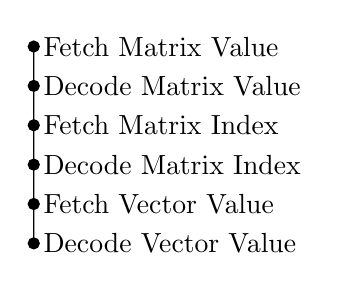
\begin{tikzpicture}
				\filldraw
					(0,2.5) circle (2pt) node[right] {Fetch Matrix Value} --
					(0,2.0) circle (2pt) node[right] {Decode Matrix Value} --
					(0,1.5) circle (2pt) node[right] {Fetch Matrix Index} --
					(0,1.0) circle (2pt) node[right] {Decode Matrix Index} --
					(0,0.5) circle (2pt) node[right] {Fetch Vector Value} --
					(0,0.0) circle (2pt) node[right] {Decode Vector Value};
			\end{tikzpicture}
			\caption{Serial Model.}
		\end{subfigure}
		\begin{subfigure}[t]{0.65\textwidth}
			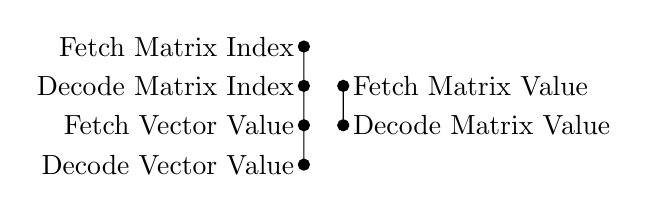
\begin{tikzpicture}
				\filldraw
					(0,2.0) circle (2pt) node[left] {Fetch Matrix Index} --
					(0,1.5) circle (2pt) node[left] {Decode Matrix Index} --
					(0,1.0) circle (2pt) node[left] {Fetch Vector Value} --
					(0,0.5) circle (2pt) node[left] {Decode Vector Value};
				\filldraw
					(0.5,1.5) circle (2pt) node[right] {Fetch Matrix Value} --
					(0.5,1.0) circle (2pt) node[right] {Decode Matrix Value};
			\end{tikzpicture}
			\caption{Parallel Model.}
		\end{subfigure}
	}
	
	\caption[Data dependency graphs for performance models.]{Comparison of the data dependency graphs used by each model, where lower nodes are dependent on higher nodes.}
	\label{fig:models-dataDeps}
\end{figure} %
Note that this model assumes that the compiler and processor can fully parallelize any operations without data dependencies, while, the instructions must be at least read serially~\cite{Hennessy:1990:ComputerArchitecture}.
Additionally, the model assumes that the bytes of each compressed value is constant, which is not true for most matrix compression and for some vector compression.
Also, the model was not used to analyze compressing multiple data structures simultaneously due to the difficulty of analyzing the resulting seven-dimension region.
Lastly, the model was used with integral values for the bytes, decode times and encode times.
The model then takes the same compression properties as the first model and computes the time to fetch and decode the values and encode the result value over 10 matrix rows with 27 entries per row.
Appendix~\ref{app:decode-model-source} contains source code for this model.

The bounds on outperforming the baseline implementation were hard to determine for the simulation model due to the nature of the model as a sum of maximizations.
However, some boundaries were computed.
Table~\ref{tab:models-singleComp} shows the restrictions when compressing only a single data structure.
\begin{table}
	\begin{tabular}{r|S|S|c}
      & {Matrix Index}  & {Matrix Value} & {Vector}\\
	{Bytes} & {Decode}        & {Decode}       & Encode and Decode \\
	\hline
	1 & 66 & 41 & \(4.75\geq 1.75\cdot\mathrm{decode}+\mathrm{encode}\)\\
	2 & 51 & 14 &\(4.75\geq 1.75\cdot\mathrm{decode}+\mathrm{encode}\)\\
	3 & 66 & 40 &\(2\geq 2\cdot\mathrm{decode}+\mathrm{encode}\)\\
	4 & 0 & 0 &\(0=\mathrm{decode}=\mathrm{encode}\) \\
	5 & {-} & 37 & \(4.75\geq 1.75\cdot\mathrm{decode}+\mathrm{encode}\)\\
	6 & {-} & 9 & Not Possible\\
	7 & {-} & 35 & \(0=\mathrm{decode}=\mathrm{encode}\)\\
	8 & {-} & 0 & \(0=\mathrm{decode}=\mathrm{encode}\)
\end{tabular}

	\caption[Simulation based model results.]{Maximum decode times in clocks for single data structure compression, according to the simulation based model.}
	\label{tab:models-singleComp}
\end{table} %
The matrix index and value columns contain the maximum time to decode a value, in clocks.
The vector column contains equations that restrict the decode and encode time, with values in clocks.
Note that the vector limits are not the only way to compute the restriction.
These compression bounds appear to be significantly related to the frequency at which multiple values are fetched from main memory simultaneously.


\section{Test Results}
\label{sec:results}
Tables~\ref{tab:results-vec}, \ref{tab:results-val} and~\ref{tab:results-ind} show the compression results for compressing just the vector values, matrix values and matrix indices respectively.
These tables contain the rating measured by HPCG, the number of iterations needed for convergence and the compression rate based on the number of cache lines fetched, which may be different then the memory allocated.
Note that some compression strategies had multiple variations that were tested.
The compression of just one data structure fails to outperform the baseline implementation; Section~\ref{sec:results-bounds} discusses this further.

\begin{table}
	\centering
	\begin{tabular}{l|S[table-format=2.6]|S[table-format=2.6]|r|c}
		            & {HPCG}   & {GFLOPs} &            & Compression \\
		Compression & {Rating} & {Rating} & Iterations & Rate \\
		\hline
		Baseline & 15.3654 & 15.7394 & 50 & 1:1 \\ %using mixed prec "all doubles" time
		Single Precision & 7.02301 & 7.10126 & 115 & 1:2 \\
		Mixed Precision & & & & \\ %b, x, d, Ad, r, z
		\hspace{3mm} \(\vec{d}\) & 5.18476 & 5.22674 & 150 & 11:12 \\
		\hspace{3mm} \(\vec{b}, \vec{x}\) & 15.3701 & 15.7503 & 50 & 5:6 \\
		\hspace{3mm} \(\vec{b}, \vec{x}, \mat{A}\vec{d}\) & 15.0428 & 15.4048 & 51 & 3:4 \\
		\hspace{3mm} \(\vec{b}, \vec{x}, \vec{d}\) & 5.20832 & 5.25084 & 150 & 3:4 \\ %using floats:b,x,d version
		\hspace{3mm} \(\vec{b}, \vec{x}, \vec{d}, \mat{A}\vec{d}\) & 5.23208 & 5.27503 & 150 & 2:3 \\
		\hspace{3mm} \(\vec{b}, \vec{x}, \vec{d}, \mat{A}\vec{d}, \vec{z}\) & 6.95894 & 7.03599 & 115 & 7:12 \\
		\hspace{3mm} \(\vec{b}, \vec{x}, \vec{d}, \vec{z}\) & 6.91343 & 6.98823 & 115 & 2:3 \\
		\hspace{3mm} \(\vec{b}, \vec{x}, \vec{z}\) & 12.2146 & 12.4516 & 64 & 3:4 \\
		%TODO consider if single b and single x should be timed seperately
		%TODO double check that single x doesn't degrade quality too much
		ZFP & & & & \\
		\hspace{3mm} 1d & & & & \\
			\hspace{6mm} 16 bits/value & 0.690138 & 0.690913 & 51 & 1:4 \\
			\hspace{6mm} 32 bits/value & 0.39397 & 0.394225 & 50 & 1:2 \\
		\hspace{3mm} 3d & & & & \\
			\hspace{6mm} 11 bits/value & NA & NA & \(\geq 500\) & 11:64 \\
			\hspace{6mm} 12 bits/value & 2.77671 & 2.78938 & 53 & 3:16 \\
			\hspace{6mm} 14 bits/value & 2.79416 & 2.80692 & 51 & 7:32\\
			%TODO get ratings for 14 bits/value
			\hspace{6mm} 16 bits/value & 2.72078 & 2.73311 & 51 & 1:4 \\
			\hspace{6mm} 24 bits/value & 2.48793 & 2.4982 & 50 & 3:8 \\ 
			\hspace{6mm} 32 bits/value & 2.17639 & 2.18425 & 50 & 1:2 \\
		SZ & & & & \\
		%timings have error setting of 1e-10 abs and 1e-10 rel
		\hspace{3mm} 7 values/block & 5.89138 & 5.94758 & 57 & 8:7 \\
		\hspace{3mm} 8 values/block & 5.78711 & 5.84115 & 57 & 1:1 to 2:1 \\
		\hspace{3mm} 12 values/block & 4.98536 & 5.02568 & 57 & 2:3 to 4:3 \\
		\hspace{3mm} 15 values/block & 4.51594 & 4.54898 & 57 & 8:15 to 16:15 \\
		\hspace{3mm} 16 values/block & 4.53536 & 4.56868 & 57 & 1:2 to 3:2 \\
		\hspace{3mm} 24 values/block & 3.67748 & 3.69907 & 57 & 1:3 to 4:3\\
		\hspace{3mm} 32 values/block & 3.1735 & 3.18973 & 57 & 1:4 to 5:4\\
	\end{tabular}
	\caption{Results of Compressing Vector Values.}
	\label{tab:results-vec}
\end{table}

\begin{table}
	\centering
	\begin{tabular}{l|S[table-format=2.6]|S[table-format=2.6]|r|c}
		            & {HPCG}   & {GFLOPs} &            & Compression \\
		Compression & {Rating} & {Rating} & Iterations & Rate \\
		\hline
		\csvreader[head to column names,separator=semicolon,filter strcmp={\type}{}]{figures/4.Results/Val.csv}{}{ \tablename & \hpcg & \gflops & \iterations & \rate \\}
		SZ & & & & \\
		\csvreader[head to column names,separator=semicolon,filter strcmp={\type}{SZ}]{figures/4.Results/Val.csv}{}{\hspace{3mm}\tablename & \hpcg & \gflops & \iterations & \rate \\}
		ZFP & & & & \\
		\csvreader[head to column names,separator=semicolon,filter strcmp={\type}{ZFP}]{figures/4.Results/Val.csv}{}{\hspace{3mm}\tablename & \hpcg & \gflops & \iterations & \rate \\}
	\end{tabular}
	\caption{Results of compressing matrix values.}
	\label{tab:results-val}
\end{table}
\begin{table}
	\centering
	\begin{tabular}{l|S[table-format=2.6]|S[table-format=2.6]|r|c}
		            & {HPCG}   & {GFLOPs} &            & Compression \\
		Compression & {Rating} & {Rating} & Iterations & Rate \\
		\hline
		\csvreader[head to column names,filter strcmp={\type}{}]{figures/4.Results/Ind.csv}{}{ \tablename & \hpcg & \gflops & \iterations & \rate \\}
		Huffman - No First Index & & & & \\
			\csvreader[head to column names,filter strcmp={\type}{huffman-nofirst}]{figures/4.Results/Ind.csv}{}{\hspace{3mm}\tablename & \hpcg & \gflops & \iterations & \rate \\}
		Huffman - First Index & & & & \\
			\csvreader[head to column names,filter strcmp={\type}{huffman-first}]{figures/4.Results/Ind.csv}{}{\hspace{3mm}\tablename & \hpcg & \gflops & \iterations & \rate \\}
		%TODO consider adding more Huffman timings (single table, cont alloc)
		Op Code & & & & \\
		\csvreader[head to column names,filter strcmp={\type}{opcode}]{figures/4.Results/Ind.csv}{}{\hspace{3mm}\tablename & \hpcg & \gflops & \iterations & \rate \\}
	\end{tabular}
	\caption{Results of Compressing Matrix Indices.}
	\label{tab:results-ind}
\end{table}

Next, combined compression schemes were tried, using SZ and single precision compression for the matrix values and using SZ, gamma and delta compression for the matrix indices.
Table~\ref{tab:results-combined} shows the results of these combined schemes.
Like the single compression tables, this table contains the rating measure by HPCG, the number of iterations needed for convergence and the cache line compression rate.
The combined scheme with the best performance used SZ compression for both values and indices.
The only other approach that outperformed the baseline implementation used 32 bit compression for the values and gamma compression for the indices.

\begin{table}
	\centering
	\begin{tabular}{l|l|S|r|c}
		\multicolumn{2}{c|}{Compression} & & & \\
		Value & Index & GFLOPs & Iterations & Compression Rate\\
		\hline
		\multicolumn{2}{c|}{Baseline} & 15.3654 & 50 & 1:1 \\
		SZ & SZ & 18.9702 & 50 & \\
		SZ & Gamma & 13.661 & 51 & \\
		SZ & Delta & 10.9903 & 50 & \\
		32 bit & SZ & 14.1796 & 51 & \\
		32 bit & Gamma & 17.6676& 51 & \\
		32 bit & Delta & 12.56 & 51 & \\
	\end{tabular}
	\caption{Results of Combined Matrix Value and Index Compression Schemes.}
	\label{tab:results-combined}
\end{table}
%TODO fill in table

\subsection{Performance Improvement Bounds}
\label{sec:results-bounds}
Note that Table~\ref{tab:results-val} shows 1 bit compression under performing the baseline implementation, even though it has a significant compression rate.
This demonstrates that compressing the matrix values alone in unable to improve performance.
For the vector values, note that the single precision implementation has a 2.3 times increase in iterations to convergence over the baseline implementation and that the GFLOPs rating of the single precision implementation is reduced by a factor of approximately 2.19 from the baseline implementation.
This hints that, even without increasing the number of Conjugate Gradient iterations, compressing the vectors requires a compression rate better than 1:2 to provide much of an improvement in performance.
This analysis is supported by the fact that none of the compression strategies tried that only compressed a single strategy where able to out perform the baseline implementation.

\subsection{Vector Compression}
%TODO start off with general info
As shown in Table~\ref{tab:results-vec}, vector compression was not successfully used to improve performance.
Section~\ref{sec:results-bounds} discusses why performance improvement is likely limited.
However, vector compression is able to make improvements when combined with other compression.
%TODO get a table reference on this, prolly the table with vec-mix+vals-SZ+inds-SZ

ZFP had poor performance when compressing vector information.
Note that 1 dimensional ZFP compression has a 16 bit granularity, and 3 dimensional ZFP compression has a 1 bit granularity~\cite{Lindstrom:2014:zfp}.
These granularity restrictions and the resulting iterations needed were used to select the tested compression rates.

SZ compression has two main configurable settings, the number of values in each block and the error bound.
There were two measures of error that were considered, absolute error and pointwise relative error.
The performance was tested with both a single error being bounded and both errors being bounded.
Absolute error is the absolute value of the difference between predicted and actual.
The pointwise relative error is the absolute error divided by the actual value.
Table~\ref{tab:results-vec} contains results for various block sizes with both an absolute error bound of \(10^{-10}\) and a pointwise relative error bound of \(10^{-10}\).
Table~\ref{tab:results-vec-SZ} contains an comparison of various error bounds for a block size of 8 values per block.
%TODO get timings with another block size (12 val blocks?)
Note that an absolute bound of \(10^{-2}\) was unable to converge within 500 iterations.
%TODO is this note useful?

\begin{table}
	\centering
	\begin{tabular}{l|S[table-format=2.6]|S[table-format=2.6]|r}
		            & {HPCG}   & {GFLOPs} &            \\
		Error Bound & {Rating} & {Rating} & Iterations \\
		\hline
		\(10^{-2}\) relative & 3.66859 & 3.69056 & 69 \\
		\(10^{-6}\) relative & 5.7806 & 5.83461 & 57 \\
		\(10^{-10}\) relative & 5.82527 & 8.87961 & 57 \\
		\(10^{-14}\) relative & 5.81357 & 5.8677 & 57 \\
		\(10^{-18}\) relative & 5.73277 & 5.78596 & 57 \\
		\(10^{-2}\) absolute & {NA} & {NA} & \(\geq 500\) \\
		\(10^{-6}\) absolute & 4.51827 & 4.55158 & 57 \\
		\(10^{-10}\) absolute & 5.14058 & 5.18313 & 57\\
		\(10^{-14}\) absolute & 5.64338 & 5.69436 & 57 \\
		\(10^{-18}\) absolute & 5.81642 & 5.87097 & 57 \\
		\(10^{-2}\) absolute and \(10^{-10}\) relative & 5.75538 & 5.809 & 57 \\
		\(10^{-10}\) absolute and \(10^{-2}\) relative & 5.22592 & 5.27053 & 57 \\
		\(10^{-10}\) absolute and \(10^{-10}\) relative & 5.78711 & 5.84115 & 57 \\
%		\(10^{-2}\) absolute or \(10^{-10}\) relative & 5.77713 & 5.83097 & 57 \\
%		\(10^{-10}\) absolute or \(10^{-2}\) relative & 5.16793 & 5.21054 & 57 \\
%		\(10^{-10}\) absolute or \(10^{-10}\) relative & 5.80555 & 5.86009 & 57 \\
	\end{tabular}
	\caption[Performance of SZ compressed vectors versus minimum error.]{Results of compressing vector values with SZ compression using various error bounds.}
	\label{tab:results-vec-SZ}
\end{table}

\subsection{Compiler Settings Analysis}
%TODO discuss why compiler settings don't have a significant affect on things

\subsection{Testing Environment}
%TODO test setup
Timings measured with a problem of size \(96^3\) with 60 processes on the walbert cluster.

\section{Conclusions}

%TODO conclusions and future work

%TODO make some notes about how SZ compression is highly dependant on matrix content while 32bitVals+gammaInds will have a more constant compression rate

\bibliography{bibliograph}

\appendix

\section{Performance Model Source Code}
\label{app:decode-model-source}
Below is the implementation of the simulation-based performance model.
The model was implemented in Common Lisp and used with Steel Bank Common Lisp version 1.4.0.

\begin{lstlisting}[language=Lisp,
					showstringspaces=false,
					numbers=left,
					numberstyle=\tiny]
;;; Global Variables

; Cluster properties
(defparameter *l1-time* 5)
(defparameter *l2-time* 12)
(defparameter *main-mem-time* 1656/10)

; Model parameters
(defparameter *rows-to-check* 128)

; Default compression settings
(defparameter *bytes-per-mat-ind* 4)
(defparameter *bytes-per-mat-val* 8)
(defparameter *bytes-per-vect* 8)
(defparameter *inds-decode-time* 0)
(defparameter *vals-decode-time* 0)
(defparameter *vect-decode-time* 0)
(defparameter *vect-encode-time* 0)


;;; Model Implementation

(defmethod fetch ((obj (eql :mat-inds)) (i integer))
  "Computes the cost of fetching the ith matrix index"
  (if (/= (floor (* (1- i) *bytes-per-mat-ind*) 64)
          (floor (* i *bytes-per-mat-ind*) 64))
    *main-mem-time*
    *l1-time*))

(defmethod fetch ((obj (eql :mat-vals)) (i integer))
  "Computes the cost of fetching the ith matrix value"
  (if (/= (floor (* (1- i) *bytes-per-mat-val*) 64)
          (floor (* i *bytes-per-mat-val*) 64))
    *main-mem-time*
    *l1-time*))

(defmethod fetch ((obj (eql :vect)) (i integer))
  "Computes the code of fetching the ith vector value"
  (cond
    ; 2/3rds of values were used by the previous index
    ((/= (mod i 3) 2) *l1-time*)
    ; 2/9ths of values were used by y-1
    ((< (/ i 3) 6) *l2-time*)
    ; 1/9th of values are being used for the first time
    (t (if (/= (floor (* (1- (/ i 27)) *bytes-per-vect*)
                      64)
               (floor (* (/ i 27) *bytes-per-vect*)
                      64))
         *main-mem-time*
         *l1-time*))))


(defun 1-row ()
  "Computes the average cost to load a row.
   *rows-to-check* provides the number of rows to use"
  (+ (/ (loop
          :for i :from 0 :below (* *rows-to-check* 27)
          :for inds-fetch-time = (fetch :mat-inds i)
          :for vals-fetch-time = (fetch :mat-vals i)
          :for vect-fetch-time = (fetch :vect i)
          :for total-vals-time = (+ vals-fetch-time
                                    *vals-decode-time*)
          :for total-vect-time = (+ inds-fetch-time
                                    *inds-decode-time*
                                    vect-fetch-time
                                    *vect-decode-time*)
          :summing (min total-vals-time total-vect-time))
        *rows-to-check*)
     *vect-encode-time*))


(defun 1-row-with-props (ind-size val-size vect-size
                         ind-decode val-decode
                         vect-decode vect-encode)
  "Like 1-row, but sets the compression properties"
  (let ((*bytes-per-mat-ind* ind-size)
        (*bytes-per-mat-val* val-size)
        (*bytes-per-vect* vect-size)
        (*inds-decode-time* ind-decode)
        (*vals-decode-time* val-decode)
        (*vect-decode-time* vect-decode)
        (*vect-encode-time* vect-encode))
    (1-row)))


\end{lstlisting}
 

\end{document}